\begin{itemize}
    \item 
    \item
\end{itemize}  


\begin{figure}[H]
    \centering
    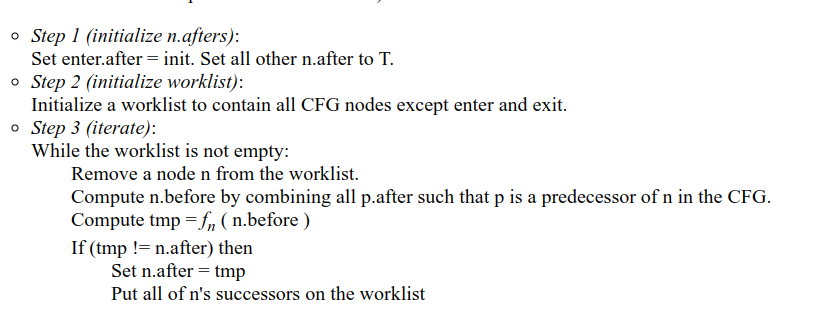
\includegraphics[width=0.4\textwidth]{p210.png}
    \caption{Iterative Algorithms}
    \label{fig:p210}
\end{figure}

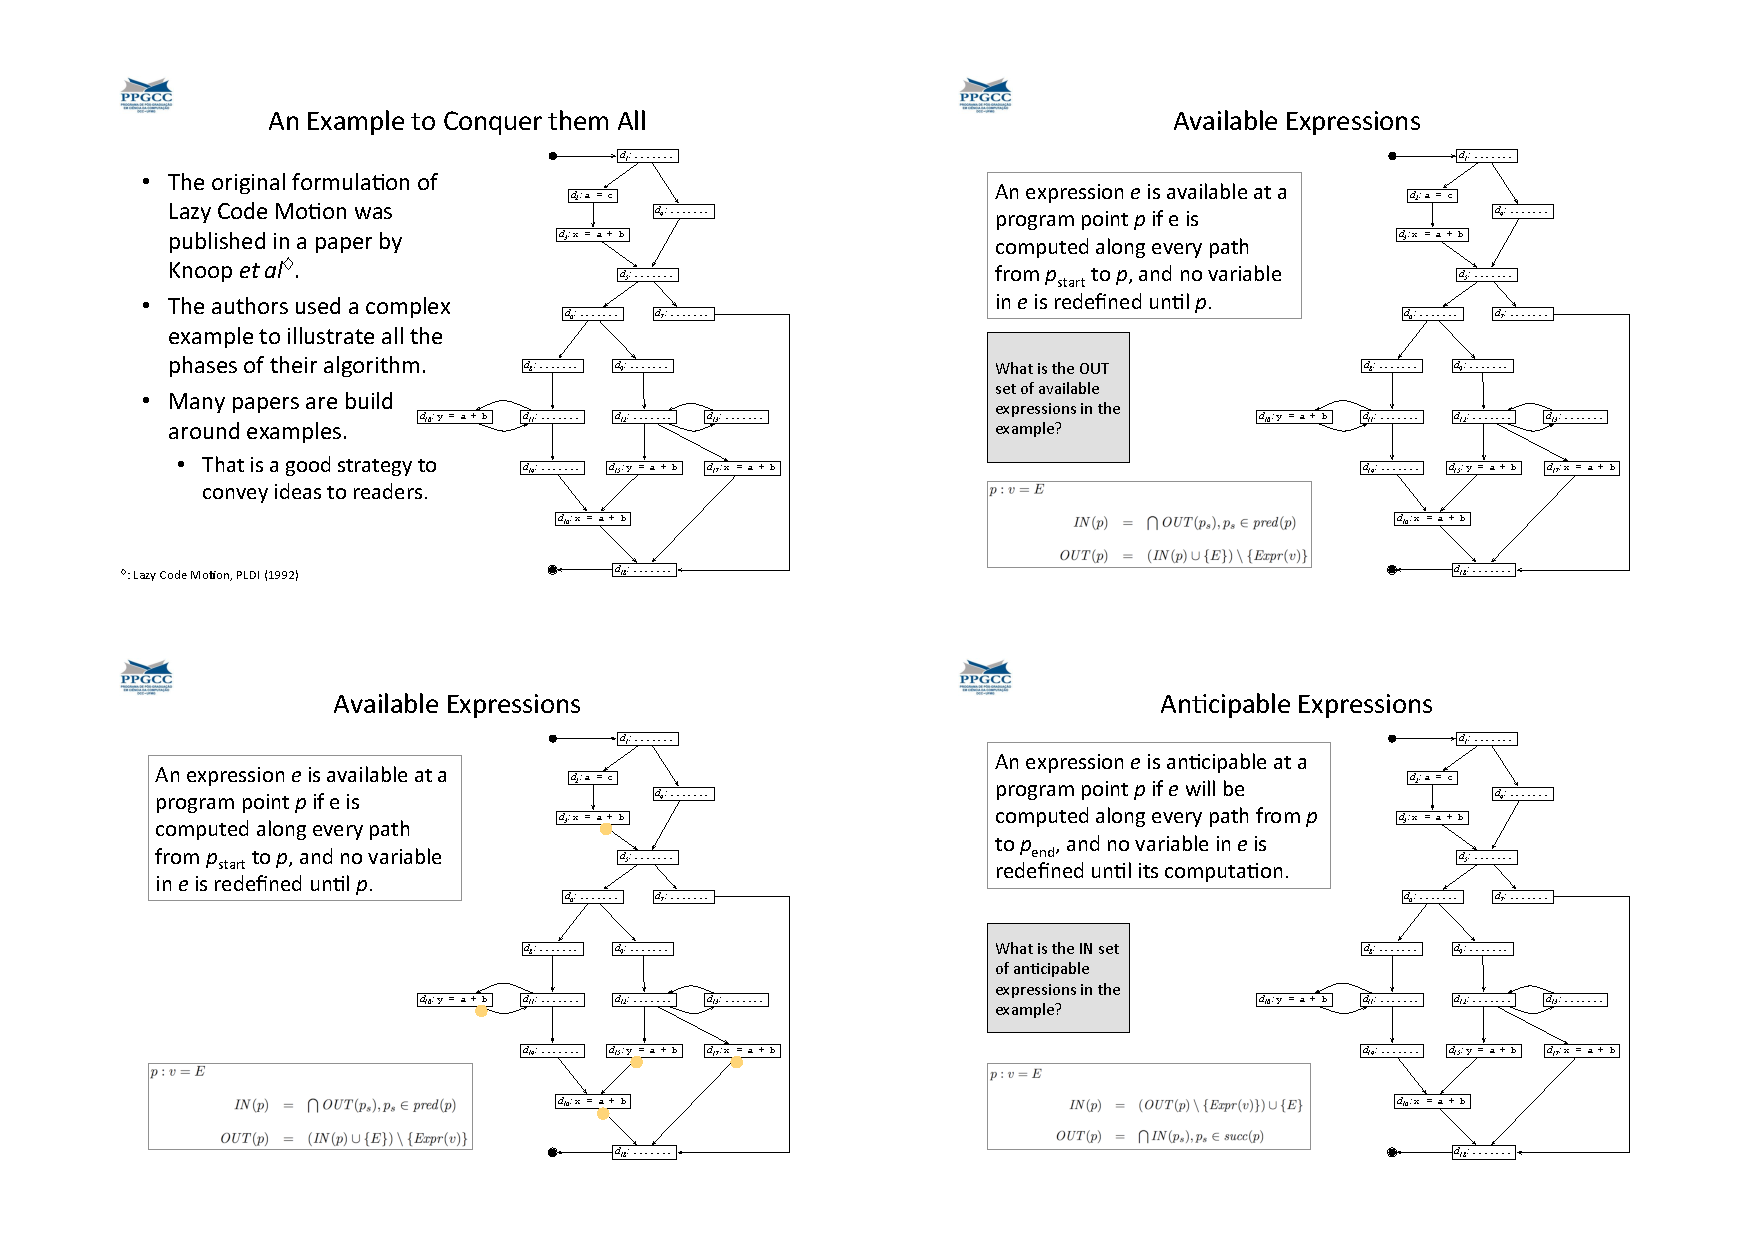
\includepdf[pages={1-}]{p99.pdf}


\begin{algorithm}
    \caption{Iterated path-convergence criterion}\label{alg:Iterated path-convergence criterion}
    \begin{algorithmic}
    
    \While{there are nodes $x, y, z$ satisfying conditions 1–5
    and \\ $z$ does not contain a $\Phi$-function for a}
    \State  insert a $\leftarrow$ $\Phi$(a, a, . . . , a) at node Z
    \EndWhile
    \end{algorithmic}
    \end{algorithm}


    \begin{figure}[H]
        \centering
        \begin{subfigure}{0.3\textwidth}
        \centering
            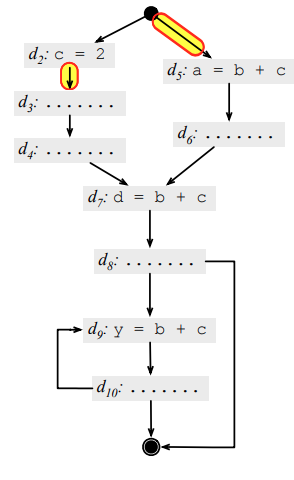
\includegraphics[width=\textwidth]{p94.png}
            \caption{For \texttt{b+c}, 	two	
            earliest	placement	
            points is colored in red.}
            \label{fig:p94}
        \end{subfigure}
        \begin{subfigure}{0.4\textwidth}
        \centering
            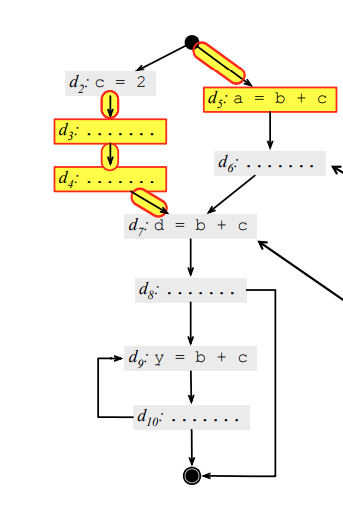
\includegraphics[width=\textwidth]{p95.png}
            \caption{For \texttt{b+c}, Latest placement edhes and blocks.}
            \label{fig:p95}
        \end{subfigure}
        
        \caption{}
           \label}
    \end{figure}
    

    \begin{lstlisting}[language=C,frame=single, caption=An simple example containing some expressions ,label = lst:expression1]

    \end{lstlisting}
    